\section{Vistas Archimate}

A continuación se muestran las vistas generadas por los autores para la muestra de la arquitectura modelada sobre Archimate 2.0. En el capítulo de anexos, en la sección \ref{app:anexo_artefactos}, se puede consultar la descripción de los artefactos que en cada una de ellas aparece.

\subsection{Vistas generales}

Seguido se presentan las vistas de Archimate que no tienen una capa específica asignada.

\subsubsection{Actores y Roles}

\begin{figure}[!htb]
  \begin{center}
    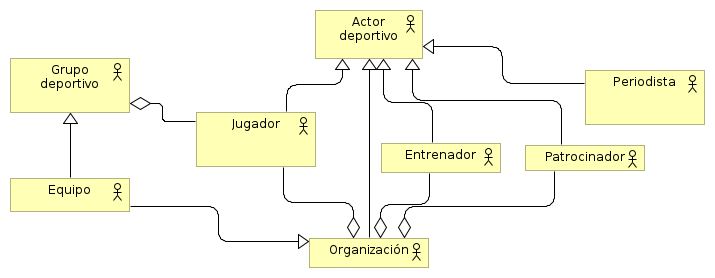
\includegraphics[width=11cm]{./imagenes/Archimate/vistas/generales/actores.png}
    \caption{Actores}
    \label{fig:Actores}
    \textbf{Fuente:}  Autores \\
    \textbf{Ver anexo en:} /Proyecto/imagenes/Archimate/vistas/generales/actores.png
  \end{center}
\end{figure}

Aunque esta no es una vista Archimate, haciendo uso de esta es posible observar los actores tenidos en cuenta en la creación del SNS. Un actor deportivo es quien desencadena a los demás actores que pueden desenvolverse en la red social debido a las funcionalidades pensadas para ella. El único actor que no ha sido propiamente pensado para ser soportado por la red social, pero que se hace necesario a la hora de tener en claro el negocio, es el periodista. El resto, en su totalidad, son soportados por la red social.

\begin{figure}[!htb]
  \begin{center}
    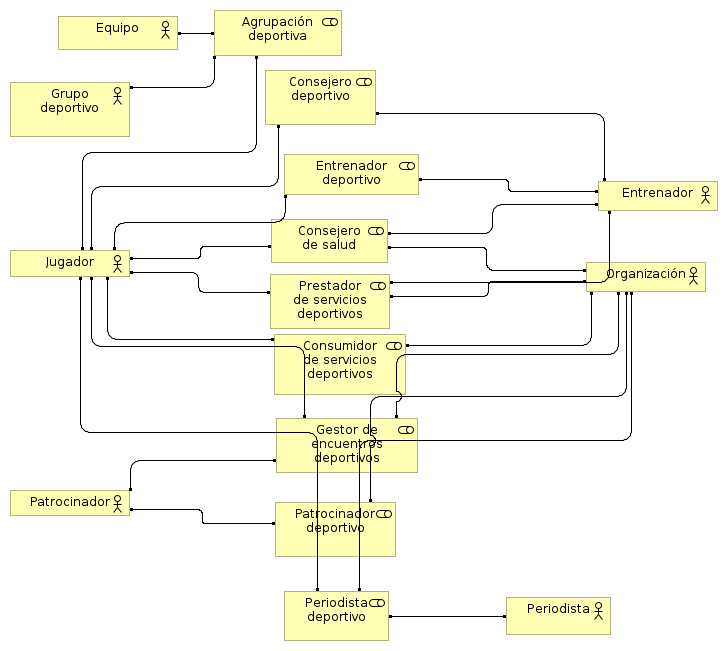
\includegraphics[width=11cm]{./imagenes/Archimate/vistas/generales/roles.png}
    \caption{Roles}
    \label{fig:Roles}
    \textbf{Fuente:}  Autores \\
    \textbf{Ver anexo en:} /Proyecto/imagenes/Archimate/vistas/generales/roles.png
  \end{center}
\end{figure}

Es una versión pequeña de un punto de vista organizacional en el que solo se intenta mostrar la relación de asignación entre actores y roles identificados en el diseño de la arquitectura. Debido a la complejidad de una red social deportiva, es posible que un actor adquiera todos los roles mostrados en la vista, sin embargo, especializandose en unos o accediendo principalmente a un rol. Tal es el caso de los roles de agrupación deportiva, entrenador deportivo, prestador de servicios deportivos y patrocinador deportivo.

\subsubsection{Introductory viewpoint}

\begin{figure}[!htb]
  \begin{center}
    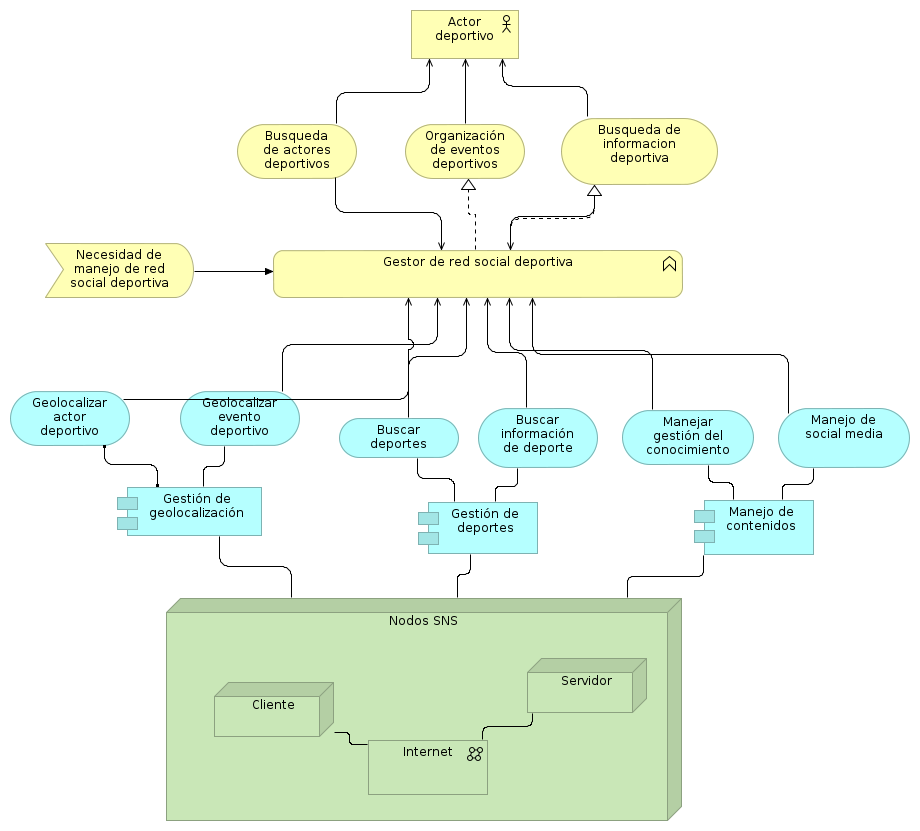
\includegraphics[width=11cm]{./imagenes/Archimate/vistas/generales/introductory.png}
    \caption{Punto de vista introductorio}
    \label{fig:introductory}
    \textbf{Fuente:}  Autores \\
    \textbf{Ver anexo en:} /Proyecto/imagenes/Archimate/vistas/generales/introductory.png
  \end{center}
\end{figure}

Esta vista muestra las principales características ofrecidas por la red social. Así, es visto que el SNS buscará, en específico, cumplir las funciones de geolocalización, del soporte de información acerca de un deporte, del manejo de social media (esto es, el despliegue de funciones para interactuar con otros en la red social) y el módulo de gestión del conocimiento (similar a la gestión de una comunidad/foro en internet).

\subsubsection{Layered viewpoint}

\begin{figure}[!htb]
  \begin{center}
    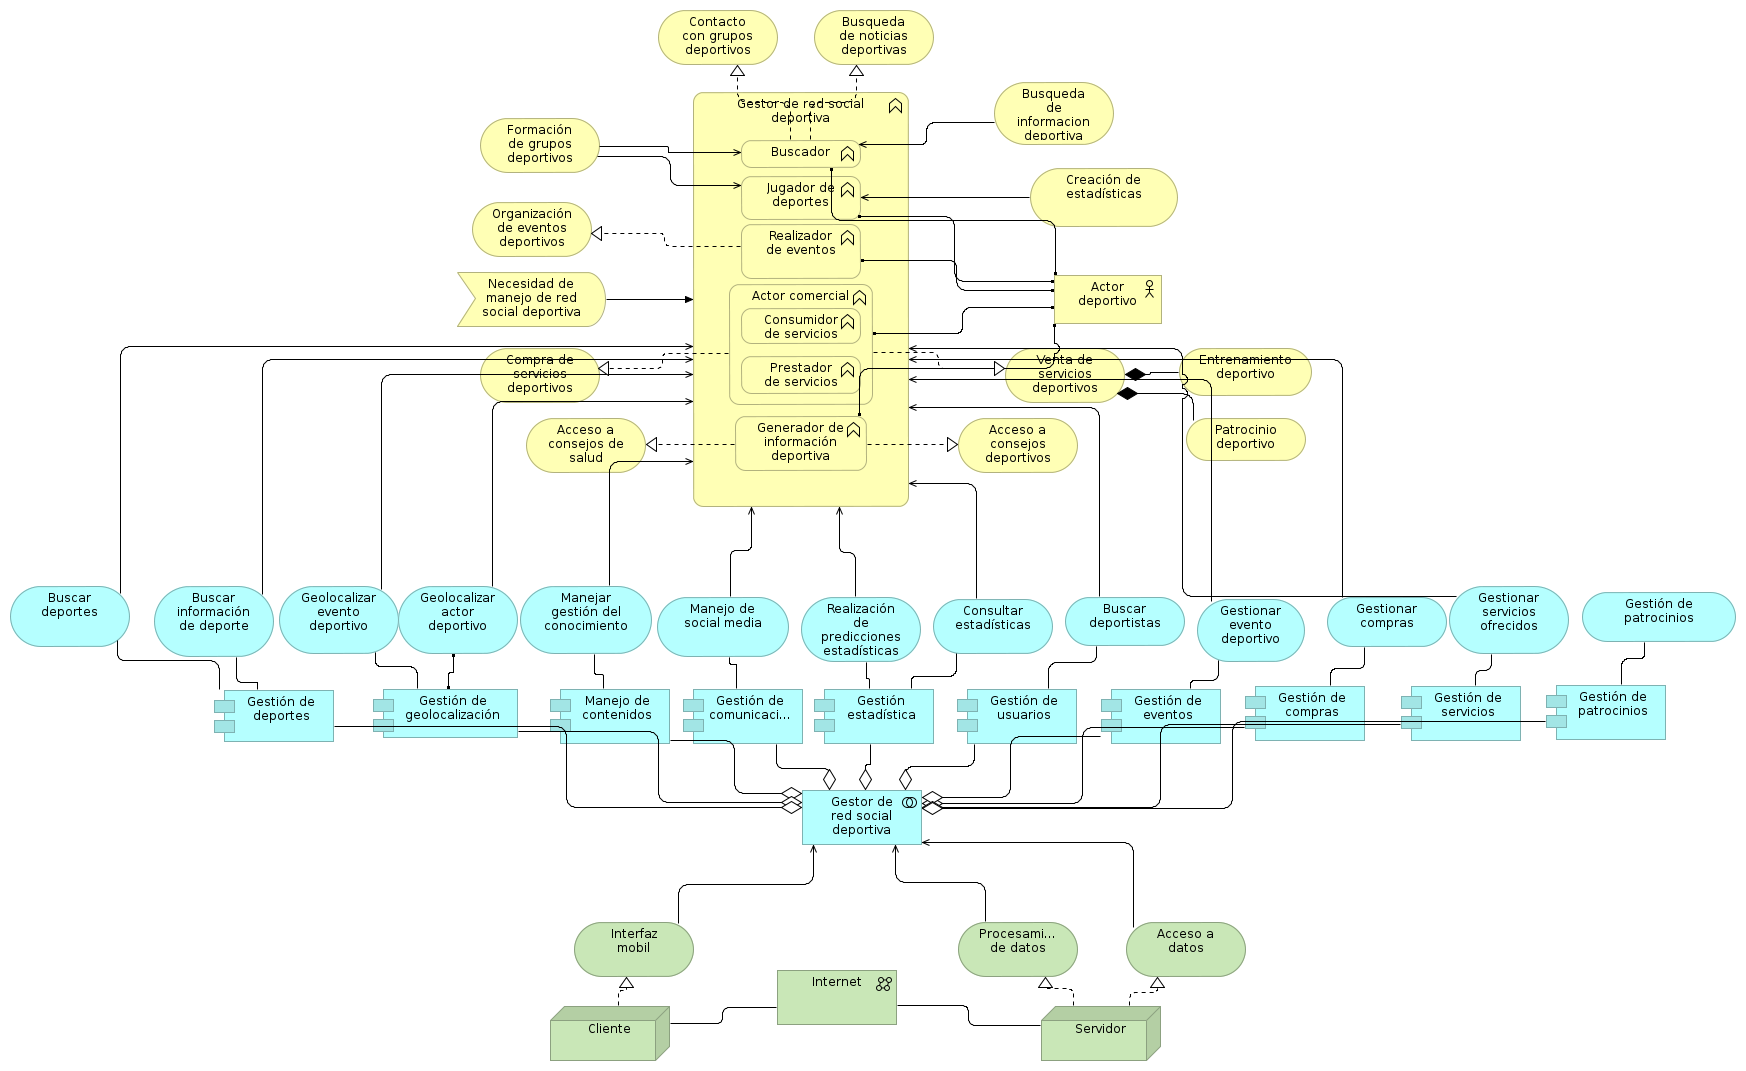
\includegraphics[width=11cm]{./imagenes/Archimate/vistas/generales/generallayered.png}
    \caption{Punto de Vista General por Capas}
    \label{fig:general_layered}
    \textbf{Fuente:}  Autores \\
    \textbf{Ver anexo en:} /Proyecto/imagenes/Archimate/vistas/generales/generallayered.png
  \end{center}
\end{figure}

Este punto de vista es una ampliación del punto de vista introductorio. En este punto de vista es posible observar la visión que han tenido los autores para mostrar una red social deportiva real, todaus las funciones que cumple y servicios que realiza/consume un actor deportivo sobre la red. A su vez, es posible observar la ampliación y la aparición de nuevas funcionalidades que soportaría el SNS, teniendo como base la orientación de la red social al deporte amateur o en camino de ser profesional. Entre las nuevas funcionalidades puede observarse la gestión de patrocinios deportivos, la gestión de compra/venta sobre el SNS, la realización de predicciones estadísticas (y, por ende, la producción de las estadísticas mismas) de eventos deportivos y actores deportivos en la red social y la gestión de eventos deportivos. En cuanto al elemento ampliado, se puede observar la ampliación de la geolocalización al ambito de los actores deportivos en la red social así como también de los eventos que en ella se produzcan.

En la capa tecnológica puede observarse la arquitectura cliente/servidor sobre internet, teniendo como terminales los dispositivos móbiles que, en este caso, serán dispositivos Android.

\subsection{Business Functions Viewpoints}

\subsubsection{Organización de Eventos Deportivos}



En este punto de vista se puede observar el paso de información a través de los diferentes roles que interactúan en la creación y ejecución de un evento deportivo (patrocinadores, agrupaciones deportivas y gestores de encuentros deportivos) quienes intercambian la información de cada uno para ser patrocinado, para pedir participación o para participar en el evento deportivo.

\clearpage

\newpage

\begin{landscape}

\begin{figure}[!htb]
  \begin{center}
    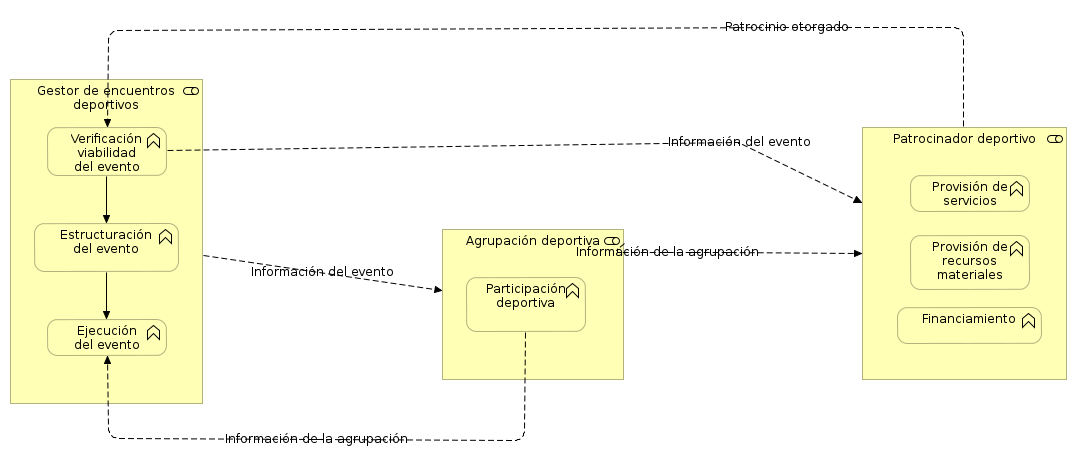
\includegraphics[width=11cm]{./imagenes/Archimate/vistas/business_functions/organizacioneventosdeportivos.png}
    \caption{Organización de Eventos Deportivos}
    \label{fig:bf_organizacion_eventos_deportivos}
    \textbf{Fuente:}  Autores \\
    \textbf{Ver anexo en:} /Proyecto/imagenes/Archimate/vistas/business\_functions/
    organizacioneventosdeportivos.png
  \end{center}
\end{figure}

\end{landscape}

\newpage

\subsubsection{Buscador Deportivo}

\begin{figure}[!htb]
  \begin{center}
    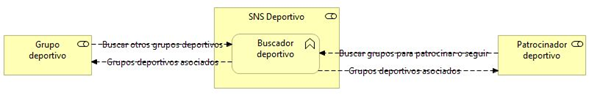
\includegraphics[width=11cm]{./imagenes/Archimate/vistas/business_functions/buscadordeportivo.png}
    \caption{Buscador deportivo}
    \label{fig:BF_BuscadorDeportivo}
    \textbf{Fuente:}  Autores \\
    \textbf{Ver anexo en:} /Proyecto/imagenes/Archimate/vistas/business\_functions/
    buscadordeportivo.png
  \end{center}
\end{figure}

En esta vista se puede observar como los roles de Grupo deportivo, Patrocinador deportivo, Coaching, Estadista deportivo, Gestor de encuentros deportivos, periodista deportivo y prestador de servicios deportivo están en capacidad de obtener y buscar información acerca de otros grupos deportivos que existan.

\subsubsection{Localización}

\begin{figure}[!htb]
  \begin{center}
    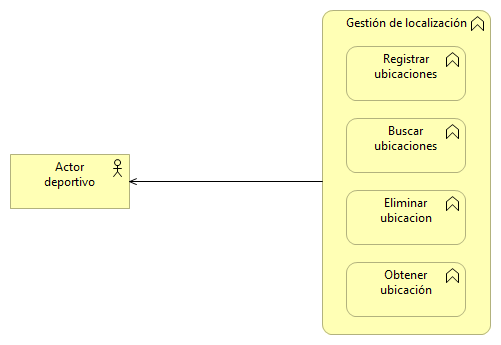
\includegraphics[width=11cm]{./imagenes/Archimate/vistas/business_functions/localizacion.png}
    \caption{Localizacion}
    \label{fig:BF_localizacion}
    \textbf{Fuente:}  Autores \\
    \textbf{Ver anexo en:} /Proyecto/imagenes/Archimate/vistas/business\_functions/
    localizacion.png
  \end{center}
\end{figure}

En esta vista se ven las funciones a las que un actor deportivo (usuario de la aplicación) tiene acceso. Tambien cabe notar que estas funciones serán utilizadas por diferentes módulos de la aplicación (self-sharing, por ejemplo) para proveer mayor funcionalidad a los usuarios.

\subsection{Business Process Viewpoints}

\subsubsection{Organización de Eventos Deportivos}

\begin{figure}[!htb]
  \begin{center}
    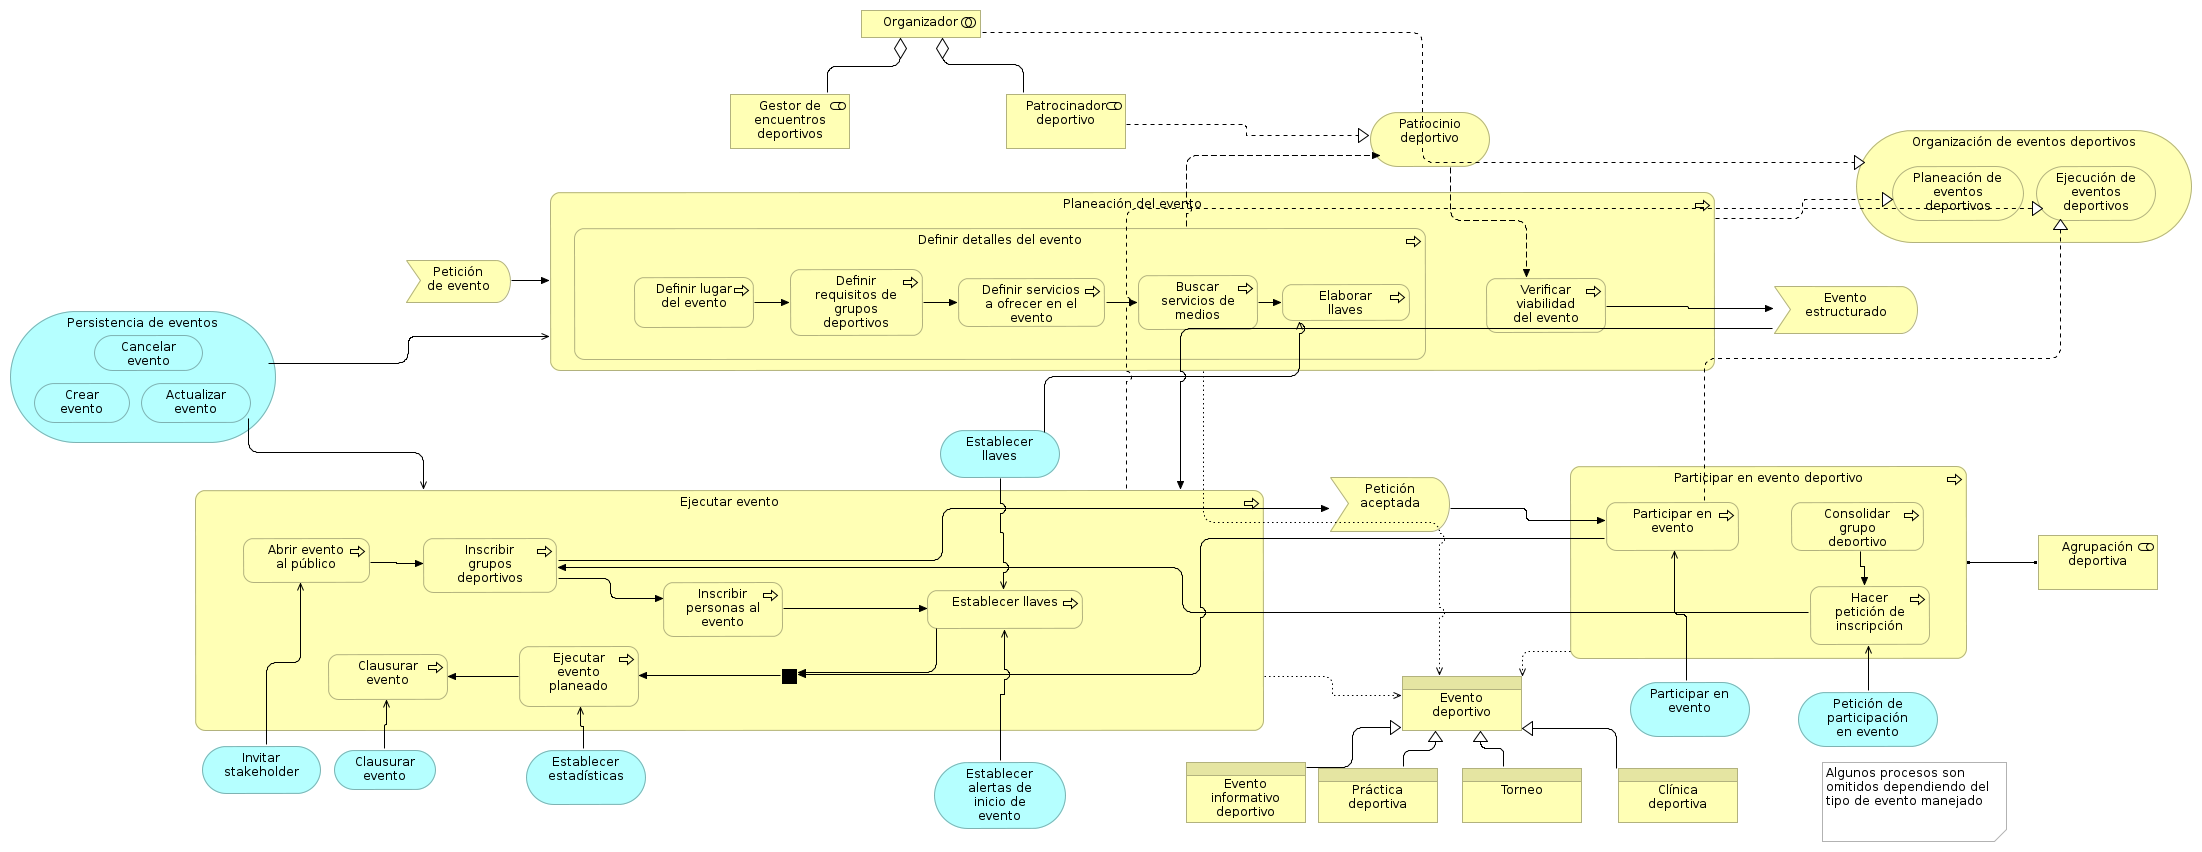
\includegraphics[width=11cm]{./imagenes/Archimate/vistas/business_process/organizacioneventosdeportivos.png}
    \caption{Organización de Eventos Deportivos}
    \label{fig:bp_organizacion_eventos_deportivos}
    \textbf{Fuente:}  Autores \\
    \textbf{Ver anexo en:} /Proyecto/imagenes/Archimate/vistas/business\_process/
    organizacioneventosdeportivos.png
  \end{center}
\end{figure}

En cuanto al proceso de organización de eventos deportivos, los autores han decidido dividir éste en tres procesos grandes: Planear el proyecto, ejecutar el proyecto y participación en el evento deportivo. Se puede ver también que un gestor de eventos deportivos puede trabajar a la par con un patrocinador deportivo para organizar el evento deportivo, con lo cual se puede discernir la conexión entre un patrocinio al evento deportivo y la organización del mismo. El primer gran proceso es soportado por servicios que proporcionan capacidades para tratar con los datos del evento; del segundo gran proceso se soportan algunos de los subprocesos pertenecientes a este, los que son considerados valiosos para el desarrollo del SNS como la invitación y notificación a participantes, así como también la clausura de un evento y la gestión de formatos deportivos; en el tercer gran proceso solo se tienen servicios para la petición a participar en el evento o la participación en el evento mismo.

\subsubsection{Buscador deportivo}

\begin{figure}[!htb]
  \begin{center}
    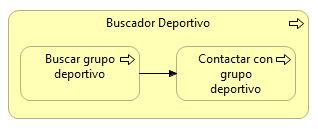
\includegraphics[width=11cm]{./imagenes/Archimate/vistas/business_process/buscadordeportivo.png}
    \caption{Buscador deportivo}
    \label{fig:BP_BuscadorDeportivo}
    \textbf{Fuente:}  Autores \\
    \textbf{Ver anexo en:} /Proyecto/imagenes/Archimate/vistas/business\_process/
    buscadordeportivo.png
  \end{center}
\end{figure}

En esta vista se muestra el proceso que se utiliza para la busqueda de grupos deportivos. Igual que en la vista anterior el proceso final (Contactar con grupo deportivo) es opcional.

\subsubsection{Localización}

\begin{figure}[!htb]
  \begin{center}
    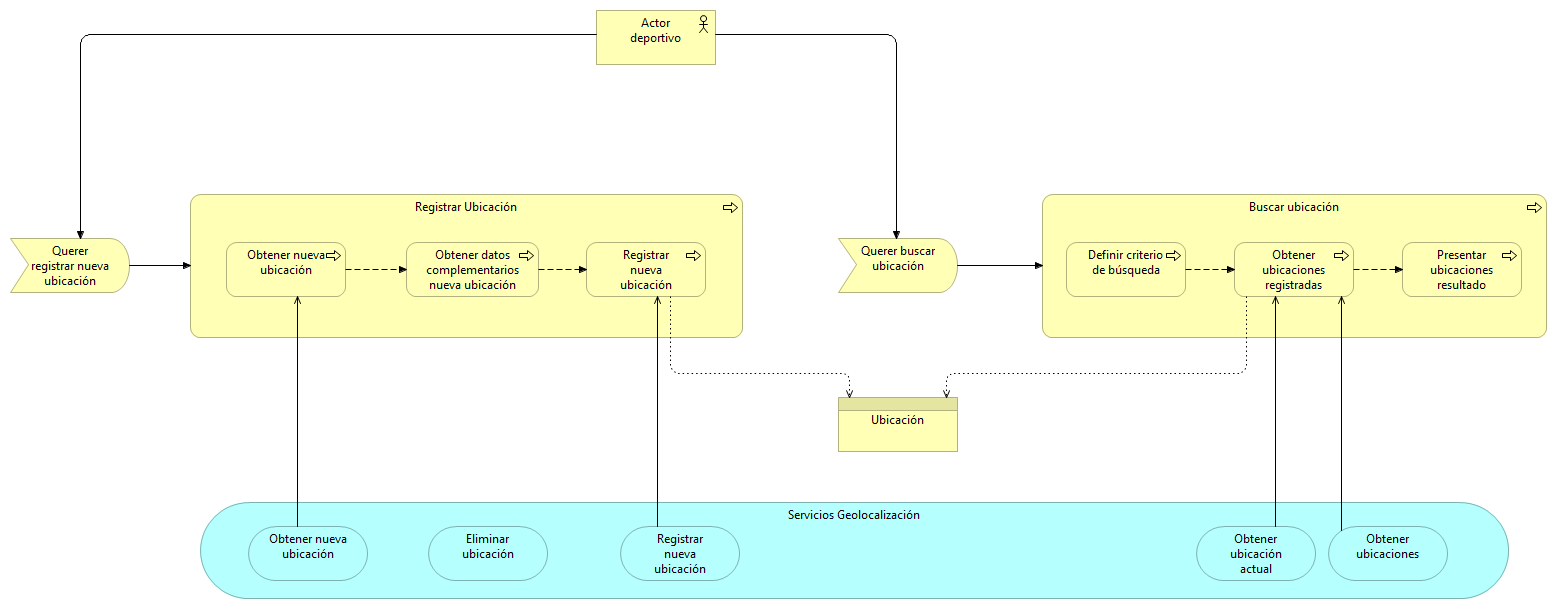
\includegraphics[width=11cm]{./imagenes/Archimate/vistas/business_process/localizacion.png}
    \caption{Localizacion}
    \label{fig:BP_localizacion}
    \textbf{Fuente:}  Autores \\
    \textbf{Ver anexo en:} /Proyecto/imagenes/Archimate/vistas/business\_process/
    localizacion.png
  \end{center}
\end{figure}

En esta vista se muestran los procesos llevados a cabo para la gestión de localización. Se presentan 2 procesos, Registrar ubicación y Buscar ubicación y se muestra como el insumo para le proceso Buscar ubicación son las ubicaciones registradas por cualquier actor deportivo de la aplicación.

\subsection{Application Usage Viewpoints}

\subsubsection{Organización de Eventos Deportivos}

\begin{figure}[!htb]
  \begin{center}
    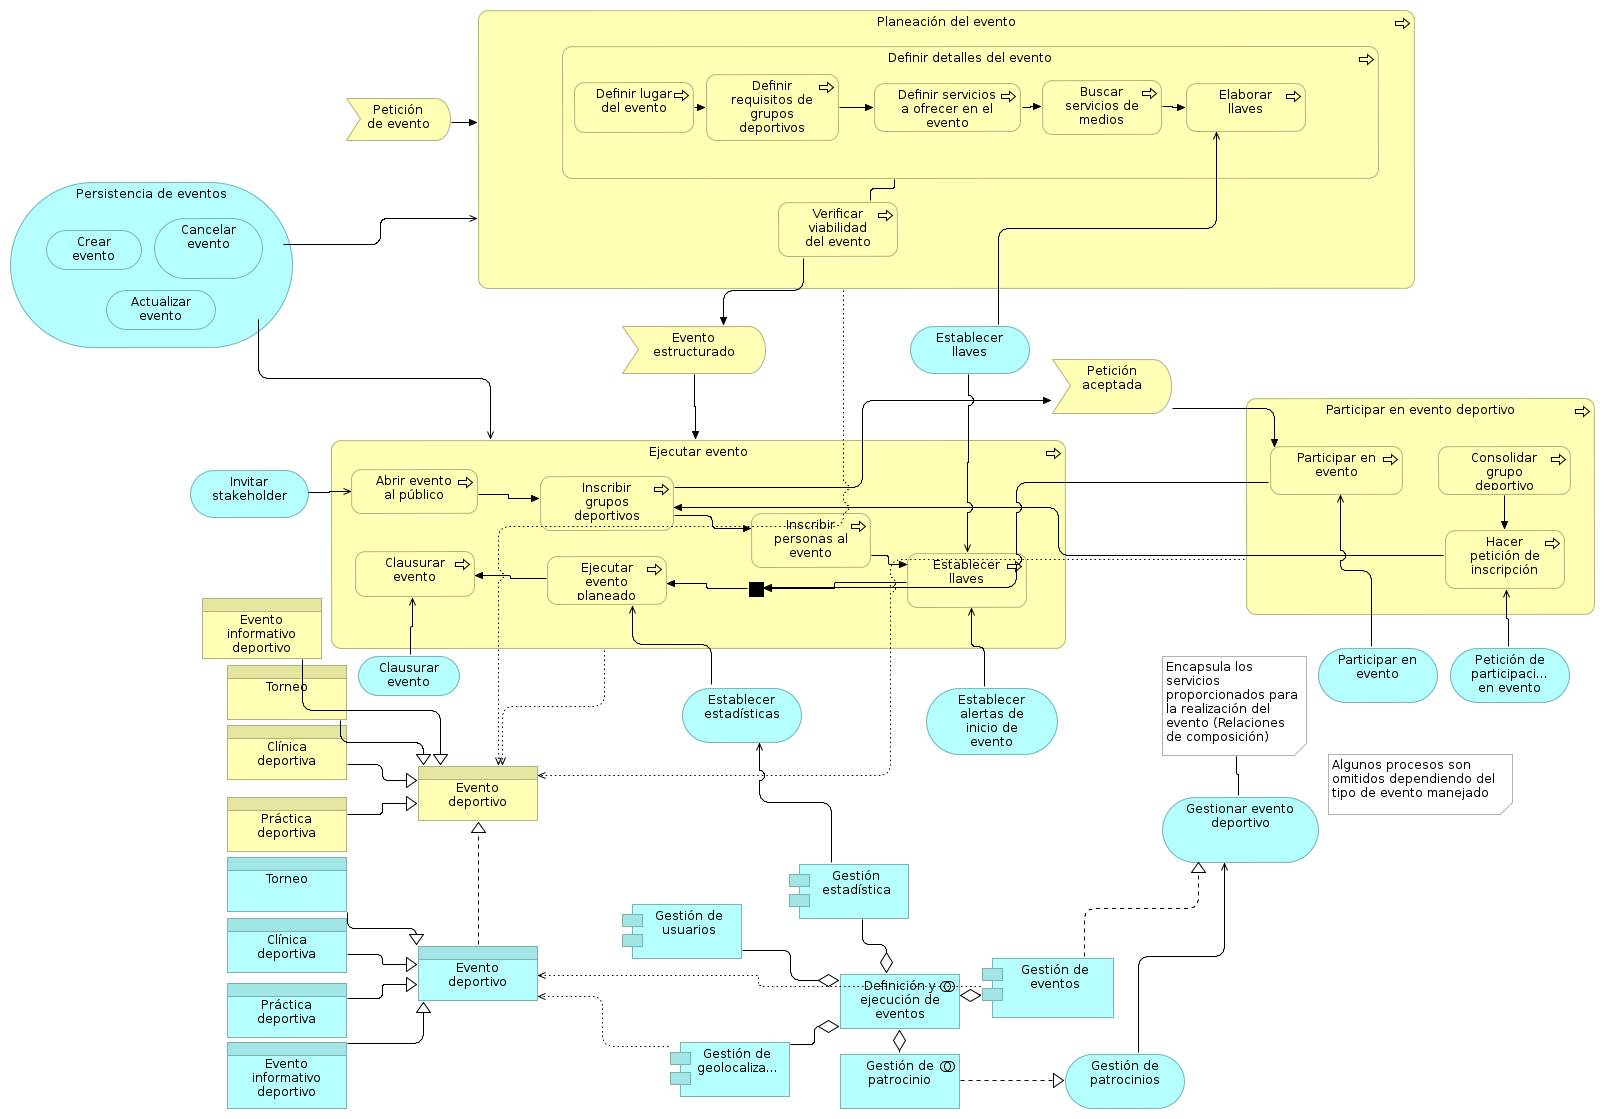
\includegraphics[width=11cm]{./imagenes/Archimate/vistas/application_usage/organizacioneventosdeportivos.png}
    \caption{Organización de Eventos Deportivos}
    \label{fig:au_organizacion_eventos_deportivos}
    \textbf{Fuente:}  Autores \\
    \textbf{Ver anexo en:} /Proyecto/imagenes/Archimate/vistas/application\_usage/
    organizacioneventosdeportivos.png
  \end{center}
\end{figure}

Para la organización de eventos deportivos, a parte de lo visto en el punto de vista de proceso de negocio, se puede observar que el SNS deportivo, en una fase final de desarrollo (más allá del prototipo que se alcanza en este proyecto), está dedicado al soporte de funcionalidades para eventos deportivos tales como torneos, clínicas, eventos informativos (como ejemplo, una conferencia deportiva) y, el elemento principal, las prácticas deportivas (prácticas informales realizadas por jugadores amateur).

En soporte de los servicios mostrados, está el componente de gestión de eventos que, junto con la gestión de patrocinio, de geolocalización, de estadísticas y de usuarios.

\subsubsection{Buscador deportivo}

\begin{figure}[!htb]
  \begin{center}
    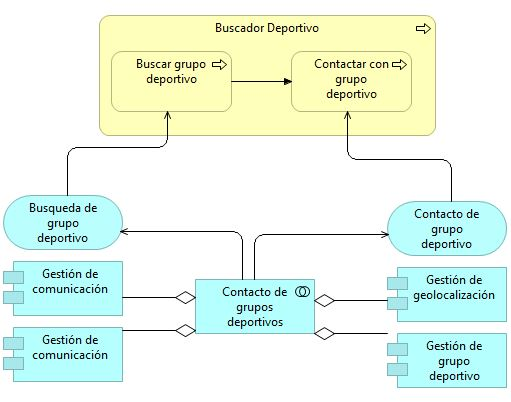
\includegraphics[width=11cm]{./imagenes/Archimate/vistas/application_usage/buscadordeportivo.png}
    \caption{Buscador deportivo}
    \label{fig:BP_BuscadorDeportivo}
    \textbf{Fuente:}  Autores \\
    \textbf{Ver anexo en:} /Proyecto/imagenes/Archimate/vistas/application\_usage/
    buscadordeportivo.png
  \end{center}
\end{figure}

De esta vista es importante resaltar la colaboración Contacto de grupos deportivos, encargada de orquestar el acceso a los componentes de Gestión de comunicación, Gestión de Geolocalización y Gestión de grupos deportivos para brindar la información necesaria en el contacto de grupos y la comunicación entre ellos.

\subsubsection{Localización}

\begin{figure}[!htb]
  \begin{center}
    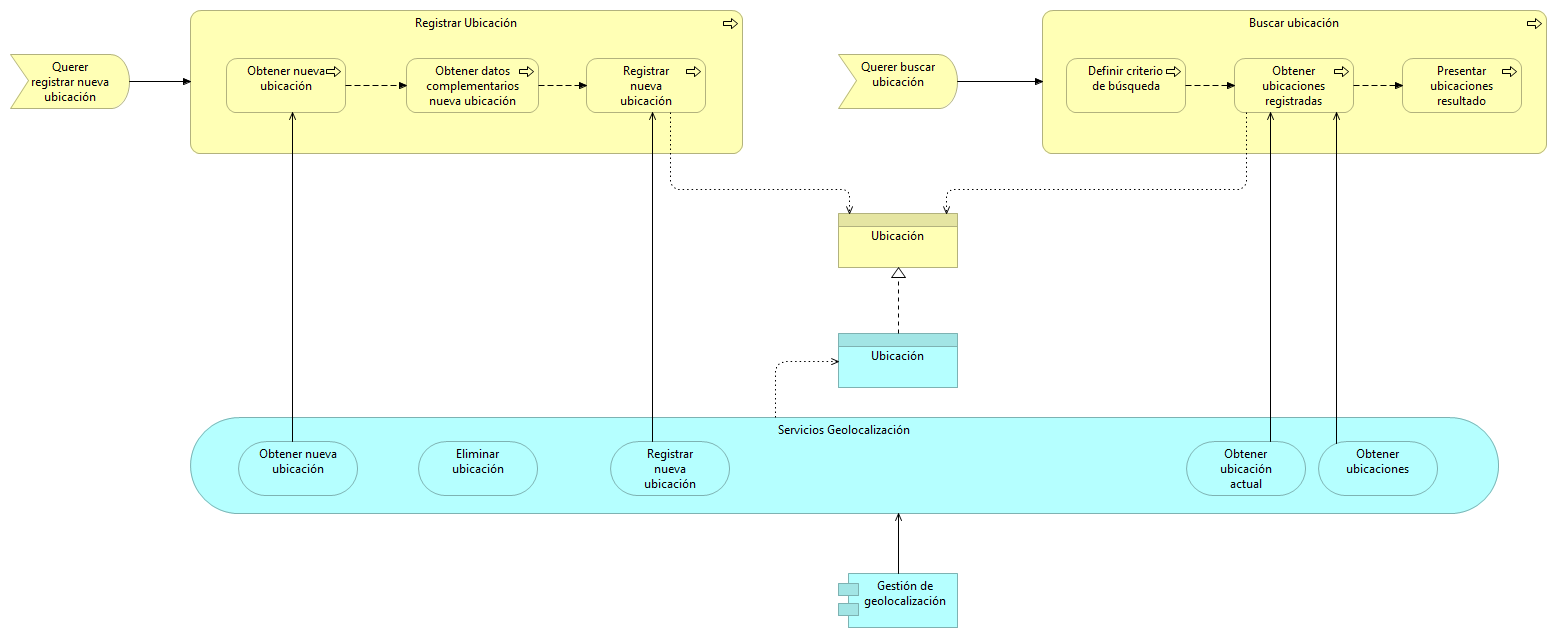
\includegraphics[width=11cm]{./imagenes/Archimate/vistas/application_usage/localizacion.png}
    \caption{Localizacion}
    \label{fig:BP_localizacion}
    \textbf{Fuente:}  Autores \\
    \textbf{Ver anexo en:} /Proyecto/imagenes/Archimate/vistas/application\_usage/
    localizacion.png
  \end{center}
\end{figure}

En esta vista se muestran los procesos llevados a cabo para la gestión de localización. Adicional a lo mostrado en la vista de proceso de negocio, se muestra el componente encargado del acceso a la base de localizaciónes de la aplicación. Estas localizaciónes son las que serán utilizadas en los demás módulos como ubicaciones, por ejemplo, para el registro de evento o lugares de práctica.

\subsection{Product Viewpoint}

\subsubsection{Product}

\begin{figure}[!htb]
  \begin{center}
    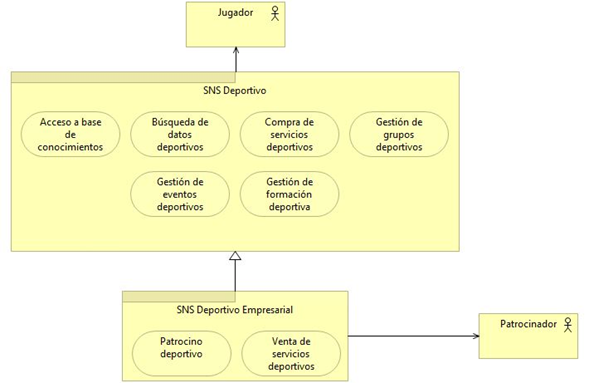
\includegraphics[width=11cm]{./imagenes/Archimate/vistas/generales/Product.png}
    \caption{Producto}
    \label{fig:Product}
    \textbf{Fuente:}  Autores \\
    \textbf{Ver anexo en:} /Proyecto/imagenes/Archimate/vistas/generales/Product.png
  \end{center}
\end{figure}

Sobre el punto de vista de productos se puede observar que productos ofrece la red social.

\subsection{Punto de vista de infraestructura}

\begin{figure}[!htb]
  \begin{center}
    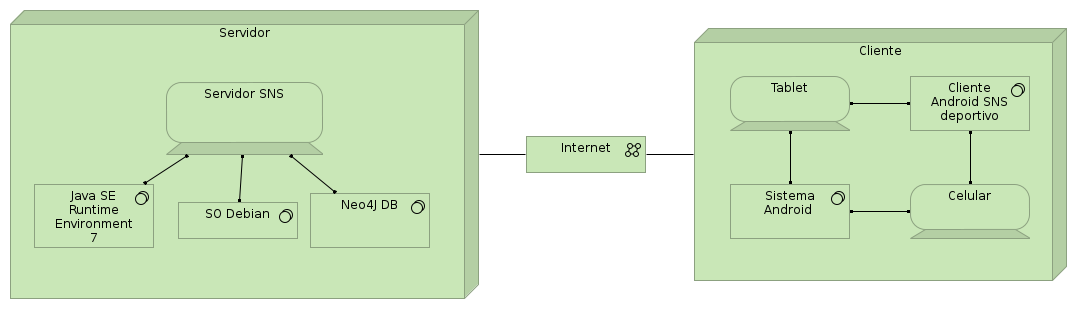
\includegraphics[width=11cm]{./imagenes/Archimate/vistas/generales/infrastructure.png}
    \caption{Punto de vista de infraestructura}
    \label{fig:infrastructure}
    \textbf{Fuente:}  Autores \\
    \textbf{Ver anexo en:} /Proyecto/imagenes/Archimate/vistas/generales/infrastructure.png
  \end{center}
\end{figure}

Sobre esta capa se puede observar que los arquitectos han decidido utilizar una arquitectura cliente/servidor para el soporte del desarrollo del SNS. A su vez, se puede observar que el software utilizado por parte del cliente deberá ser un sistema android con el cliente desarrollado específicamente para dar la GUI del SNS. Por parte del servidor se puede ver que se utilizarán entornos Java para el servidor de aplicaciones, Neo4j como la base de datos y sistema operativo Debian. Todo estará soportado sobre conexiones por medio de la red internet.